\PassOptionsToPackage{unicode=true}{hyperref} % options for packages loaded elsewhere
\PassOptionsToPackage{hyphens}{url}
%
\documentclass[ignorenonframetext,]{beamer}
\usepackage{pgfpages}
\setbeamertemplate{caption}[numbered]
\setbeamertemplate{caption label separator}{: }
\setbeamercolor{caption name}{fg=normal text.fg}
\beamertemplatenavigationsymbolsempty
% Prevent slide breaks in the middle of a paragraph:
\widowpenalties 1 10000
\raggedbottom
\setbeamertemplate{part page}{
\centering
\begin{beamercolorbox}[sep=16pt,center]{part title}
  \usebeamerfont{part title}\insertpart\par
\end{beamercolorbox}
}
\setbeamertemplate{section page}{
\centering
\begin{beamercolorbox}[sep=12pt,center]{part title}
  \usebeamerfont{section title}\insertsection\par
\end{beamercolorbox}
}
\setbeamertemplate{subsection page}{
\centering
\begin{beamercolorbox}[sep=8pt,center]{part title}
  \usebeamerfont{subsection title}\insertsubsection\par
\end{beamercolorbox}
}
\AtBeginPart{
  \frame{\partpage}
}
\AtBeginSection{
  \ifbibliography
  \else
    \frame{\sectionpage}
  \fi
}
\AtBeginSubsection{
  \frame{\subsectionpage}
}
\usepackage{lmodern}
\usepackage{amssymb,amsmath}
\usepackage{ifxetex,ifluatex}
\usepackage{fixltx2e} % provides \textsubscript
\ifnum 0\ifxetex 1\fi\ifluatex 1\fi=0 % if pdftex
  \usepackage[T1]{fontenc}
  \usepackage[utf8]{inputenc}
  \usepackage{textcomp} % provides euro and other symbols
\else % if luatex or xelatex
  \usepackage{unicode-math}
  \defaultfontfeatures{Ligatures=TeX,Scale=MatchLowercase}
\fi
\usecolortheme{beaver}
% use upquote if available, for straight quotes in verbatim environments
\IfFileExists{upquote.sty}{\usepackage{upquote}}{}
% use microtype if available
\IfFileExists{microtype.sty}{%
\usepackage[]{microtype}
\UseMicrotypeSet[protrusion]{basicmath} % disable protrusion for tt fonts
}{}
\IfFileExists{parskip.sty}{%
\usepackage{parskip}
}{% else
\setlength{\parindent}{0pt}
\setlength{\parskip}{6pt plus 2pt minus 1pt}
}
\usepackage{hyperref}
\hypersetup{
            pdftitle={Manejo de datos en R (II)},
            pdfauthor={Introducción a la Línea de Comandos para Análisis Bioinformáticos},
            pdfborder={0 0 0},
            breaklinks=true}
\urlstyle{same}  % don't use monospace font for urls
\newif\ifbibliography
\usepackage{color}
\usepackage{fancyvrb}
\newcommand{\VerbBar}{|}
\newcommand{\VERB}{\Verb[commandchars=\\\{\}]}
\DefineVerbatimEnvironment{Highlighting}{Verbatim}{commandchars=\\\{\}}
% Add ',fontsize=\small' for more characters per line
\usepackage{framed}
\definecolor{shadecolor}{RGB}{248,248,248}
\newenvironment{Shaded}{\begin{snugshade}}{\end{snugshade}}
\newcommand{\AlertTok}[1]{\textcolor[rgb]{0.94,0.16,0.16}{#1}}
\newcommand{\AnnotationTok}[1]{\textcolor[rgb]{0.56,0.35,0.01}{\textbf{\textit{#1}}}}
\newcommand{\AttributeTok}[1]{\textcolor[rgb]{0.77,0.63,0.00}{#1}}
\newcommand{\BaseNTok}[1]{\textcolor[rgb]{0.00,0.00,0.81}{#1}}
\newcommand{\BuiltInTok}[1]{#1}
\newcommand{\CharTok}[1]{\textcolor[rgb]{0.31,0.60,0.02}{#1}}
\newcommand{\CommentTok}[1]{\textcolor[rgb]{0.56,0.35,0.01}{\textit{#1}}}
\newcommand{\CommentVarTok}[1]{\textcolor[rgb]{0.56,0.35,0.01}{\textbf{\textit{#1}}}}
\newcommand{\ConstantTok}[1]{\textcolor[rgb]{0.00,0.00,0.00}{#1}}
\newcommand{\ControlFlowTok}[1]{\textcolor[rgb]{0.13,0.29,0.53}{\textbf{#1}}}
\newcommand{\DataTypeTok}[1]{\textcolor[rgb]{0.13,0.29,0.53}{#1}}
\newcommand{\DecValTok}[1]{\textcolor[rgb]{0.00,0.00,0.81}{#1}}
\newcommand{\DocumentationTok}[1]{\textcolor[rgb]{0.56,0.35,0.01}{\textbf{\textit{#1}}}}
\newcommand{\ErrorTok}[1]{\textcolor[rgb]{0.64,0.00,0.00}{\textbf{#1}}}
\newcommand{\ExtensionTok}[1]{#1}
\newcommand{\FloatTok}[1]{\textcolor[rgb]{0.00,0.00,0.81}{#1}}
\newcommand{\FunctionTok}[1]{\textcolor[rgb]{0.00,0.00,0.00}{#1}}
\newcommand{\ImportTok}[1]{#1}
\newcommand{\InformationTok}[1]{\textcolor[rgb]{0.56,0.35,0.01}{\textbf{\textit{#1}}}}
\newcommand{\KeywordTok}[1]{\textcolor[rgb]{0.13,0.29,0.53}{\textbf{#1}}}
\newcommand{\NormalTok}[1]{#1}
\newcommand{\OperatorTok}[1]{\textcolor[rgb]{0.81,0.36,0.00}{\textbf{#1}}}
\newcommand{\OtherTok}[1]{\textcolor[rgb]{0.56,0.35,0.01}{#1}}
\newcommand{\PreprocessorTok}[1]{\textcolor[rgb]{0.56,0.35,0.01}{\textit{#1}}}
\newcommand{\RegionMarkerTok}[1]{#1}
\newcommand{\SpecialCharTok}[1]{\textcolor[rgb]{0.00,0.00,0.00}{#1}}
\newcommand{\SpecialStringTok}[1]{\textcolor[rgb]{0.31,0.60,0.02}{#1}}
\newcommand{\StringTok}[1]{\textcolor[rgb]{0.31,0.60,0.02}{#1}}
\newcommand{\VariableTok}[1]{\textcolor[rgb]{0.00,0.00,0.00}{#1}}
\newcommand{\VerbatimStringTok}[1]{\textcolor[rgb]{0.31,0.60,0.02}{#1}}
\newcommand{\WarningTok}[1]{\textcolor[rgb]{0.56,0.35,0.01}{\textbf{\textit{#1}}}}
\usepackage{graphicx,grffile}
\makeatletter
\def\maxwidth{\ifdim\Gin@nat@width>\linewidth\linewidth\else\Gin@nat@width\fi}
\def\maxheight{\ifdim\Gin@nat@height>\textheight\textheight\else\Gin@nat@height\fi}
\makeatother
% Scale images if necessary, so that they will not overflow the page
% margins by default, and it is still possible to overwrite the defaults
% using explicit options in \includegraphics[width, height, ...]{}
\setkeys{Gin}{width=\maxwidth,height=\maxheight,keepaspectratio}
\setlength{\emergencystretch}{3em}  % prevent overfull lines
\providecommand{\tightlist}{%
  \setlength{\itemsep}{0pt}\setlength{\parskip}{0pt}}
\setcounter{secnumdepth}{0}

% set default figure placement to htbp
\makeatletter
\def\fps@figure{htbp}
\makeatother

\usepackage{tikz}
\usepackage{graphicx}
\usetikzlibrary{calc}
\usepackage{pgfplots}
\usepackage{environ}
\useoutertheme{miniframes}
\useinnertheme{circles}

\title{Manejo de datos en R (II)}
\author{Introducción a la Línea de Comandos para Análisis Bioinformáticos}
\date{03 de Marzo, 2020}

\begin{document}
\frame{\titlepage}

\hypertarget{dia-martes}{%
\section{Dia martes}\label{dia-martes}}

\begin{frame}{Slide con muchos tipos de graficos}
\protect\hypertarget{slide-con-muchos-tipos-de-graficos}{}

\end{frame}

\begin{frame}{Idea de lo que lleva hacer un grafico para hacerlo bien}
\protect\hypertarget{idea-de-lo-que-lleva-hacer-un-grafico-para-hacerlo-bien}{}

\end{frame}

\begin{frame}{Que hay detras de hacer estos graficos en R? Muchas
librerias, de las cuales un monton son del universo tidyverse.}
\protect\hypertarget{que-hay-detras-de-hacer-estos-graficos-en-r-muchas-librerias-de-las-cuales-un-monton-son-del-universo-tidyverse.}{}

\end{frame}

\begin{frame}{Los que no son de universo tidyverse igual tienen que ser
retocadas generalmente, so\ldots{} its good to learn tidyverse.}
\protect\hypertarget{los-que-no-son-de-universo-tidyverse-igual-tienen-que-ser-retocadas-generalmente-so-its-good-to-learn-tidyverse.}{}

\end{frame}

\begin{frame}{Cuales son las operaciones que generalmente se hacen con
los datos?}
\protect\hypertarget{cuales-son-las-operaciones-que-generalmente-se-hacen-con-los-datos}{}

\begin{itemize}
\tightlist
\item
  Cargar datos \emph{crudos}/Guardar datos finales y tablas de interés.
\item
  Filtrar datos (con criterio).
\item
  Unir datos que vienen de diferentes fuentes, referentes a un mismo
  conjunto estudiado.
\item
  Hacer modificaciones: crear \emph{tags}, correcciones ortográficas,
  filas y columnas de tablas, etc\ldots{}
\item
  Generar nuevos datos: obtener promedios, medianas, aplicar funciones
  de librerías.
\item
  Dejar anotado y reportar lo hecho.
\end{itemize}

\end{frame}

\begin{frame}{Una pequeña ilustración: es posible que querramos trabajar
con un GFF}
\protect\hypertarget{una-pequeuxf1a-ilustraciuxf3n-es-posible-que-querramos-trabajar-con-un-gff}{}

\begin{itemize}
\tightlist
\item
  Cargo un GFF
\item
  Filtro para quedarme con transcriptos codificantes
\item
  De ahí capaz quiero hacer una tabla con datos como largo de
  transcripto y contenido GC
\item
  Entonces tengo que generarme una tabla que tenga las secuencias, y
  luego unir ambas
\item
  Subsetear por transcripto , obtener el largo, y calcular GC
\item
  Capaz me armo un tag que diga si son `low GC', `medium GC' o `high
  GC'.
\item
  Después puedo llegar a querer plotear.
\end{itemize}

Y así con todos los datos que nos vamos cruzando\ldots{} nos vamos a ir
encontrando cosas que vamos a tener que hacer.

\end{frame}

\begin{frame}{Ahi recien paso a hablar del paquete}
\protect\hypertarget{ahi-recien-paso-a-hablar-del-paquete}{}

\end{frame}

\begin{frame}{Bibliografía}
\protect\hypertarget{bibliografuxeda}{}

\begin{center}
\includegraphics[width=0.45\linewidth]{cover_rfordatascience} \end{center}

\end{frame}

\begin{frame}{tidy}
\protect\hypertarget{tidy}{}

\begin{tikzpicture}[remember picture,overlay]
  \node[anchor=south west,inner sep=0pt] at ($(current page.south west)+(0cm,7.8cm)$) {
     
\includegraphics[width=1.5cm]{tidyverse.png}
  };
\end{tikzpicture}

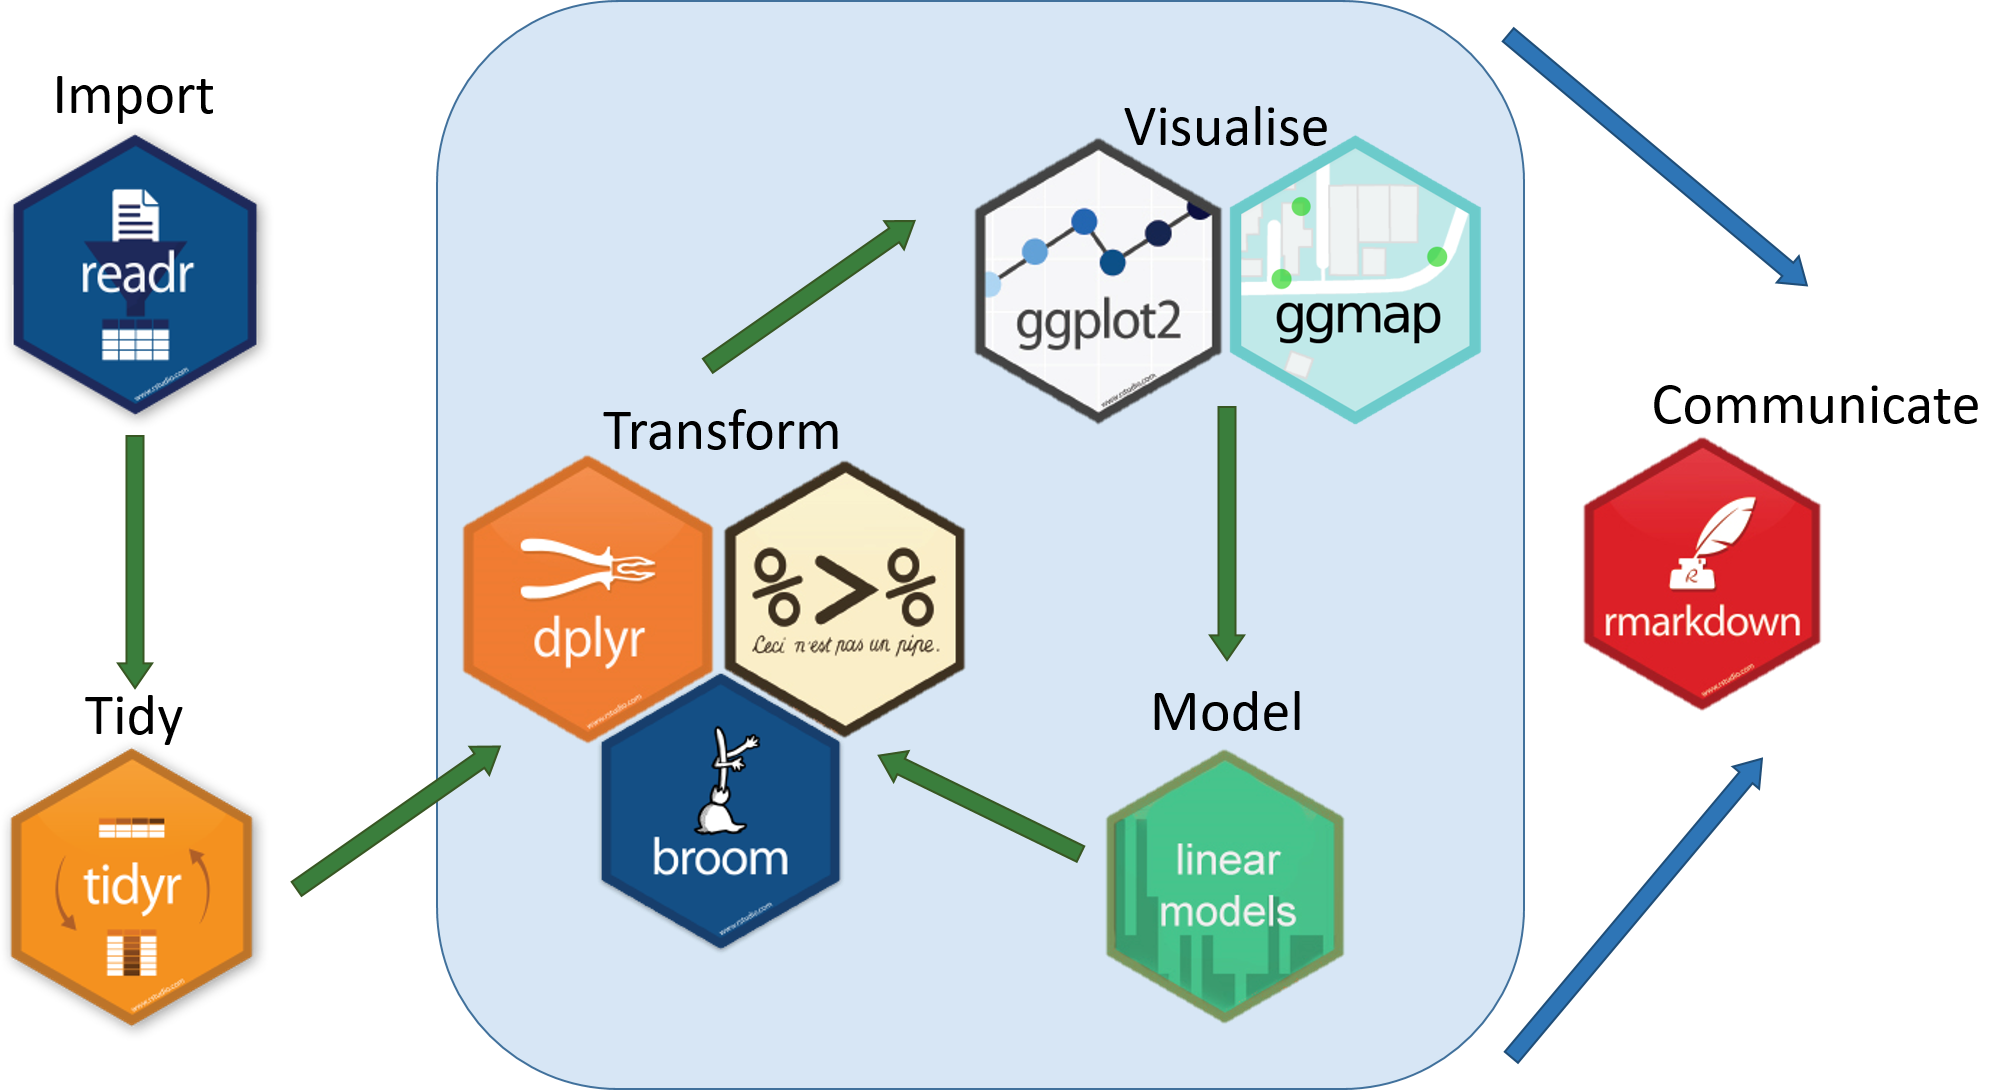
\includegraphics{tidyverse_packages.png}

\end{frame}

\begin{frame}{tibb}
\protect\hypertarget{tibb}{}

\begin{tikzpicture}[remember picture,overlay]
  \node[anchor=south west,inner sep=0pt] at ($(current page.south west)+(0cm,7.8cm)$) {
     
\includegraphics[width=1.5cm]{tibbles.png}
  };
\end{tikzpicture}

\begin{itemize}
\tightlist
\item
  Tibbles are data frames, but they tweak some older behaviours to make
  life a little easier.
\item
  Almost all of the functions that you'll use in this book produce
  tibbles, as tibbles are one of the unifying features of the tidyverse
\item
  It's possible for a tibble to have column names that are not valid R
  variable names: backtick!
\item
  Another way to create a tibble is with tribble(), short for transposed
  tibble. tribble() is customised for data entry in code: column
  headings are defined by formulas (i.e.~they start with
  \textasciitilde{}), and entries are separated by commas.
\end{itemize}

\end{frame}

\begin{frame}[fragile]{tibb}
\protect\hypertarget{tibb-1}{}

\begin{tikzpicture}[remember picture,overlay]
  \node[anchor=south west,inner sep=0pt] at ($(current page.south west)+(0cm,7.8cm)$) {
     
\includegraphics[width=1.5cm]{tibbles.png}
  };
\end{tikzpicture}

\begin{Shaded}
\begin{Highlighting}[]
\NormalTok{iris}
\end{Highlighting}
\end{Shaded}

\begin{verbatim}
##     Sepal.Length Sepal.Width Petal.Length Petal.Width    Species
## 1            5.1         3.5          1.4         0.2     setosa
## 2            4.9         3.0          1.4         0.2     setosa
## 3            4.7         3.2          1.3         0.2     setosa
## 4            4.6         3.1          1.5         0.2     setosa
## 5            5.0         3.6          1.4         0.2     setosa
## 6            5.4         3.9          1.7         0.4     setosa
## 7            4.6         3.4          1.4         0.3     setosa
## 8            5.0         3.4          1.5         0.2     setosa
## 9            4.4         2.9          1.4         0.2     setosa
## 10           4.9         3.1          1.5         0.1     setosa
## 11           5.4         3.7          1.5         0.2     setosa
## 12           4.8         3.4          1.6         0.2     setosa
## 13           4.8         3.0          1.4         0.1     setosa
## 14           4.3         3.0          1.1         0.1     setosa
## 15           5.8         4.0          1.2         0.2     setosa
## 16           5.7         4.4          1.5         0.4     setosa
## 17           5.4         3.9          1.3         0.4     setosa
## 18           5.1         3.5          1.4         0.3     setosa
## 19           5.7         3.8          1.7         0.3     setosa
## 20           5.1         3.8          1.5         0.3     setosa
## 21           5.4         3.4          1.7         0.2     setosa
## 22           5.1         3.7          1.5         0.4     setosa
## 23           4.6         3.6          1.0         0.2     setosa
## 24           5.1         3.3          1.7         0.5     setosa
## 25           4.8         3.4          1.9         0.2     setosa
## 26           5.0         3.0          1.6         0.2     setosa
## 27           5.0         3.4          1.6         0.4     setosa
## 28           5.2         3.5          1.5         0.2     setosa
## 29           5.2         3.4          1.4         0.2     setosa
## 30           4.7         3.2          1.6         0.2     setosa
## 31           4.8         3.1          1.6         0.2     setosa
## 32           5.4         3.4          1.5         0.4     setosa
## 33           5.2         4.1          1.5         0.1     setosa
## 34           5.5         4.2          1.4         0.2     setosa
## 35           4.9         3.1          1.5         0.2     setosa
## 36           5.0         3.2          1.2         0.2     setosa
## 37           5.5         3.5          1.3         0.2     setosa
## 38           4.9         3.6          1.4         0.1     setosa
## 39           4.4         3.0          1.3         0.2     setosa
## 40           5.1         3.4          1.5         0.2     setosa
## 41           5.0         3.5          1.3         0.3     setosa
## 42           4.5         2.3          1.3         0.3     setosa
## 43           4.4         3.2          1.3         0.2     setosa
## 44           5.0         3.5          1.6         0.6     setosa
## 45           5.1         3.8          1.9         0.4     setosa
## 46           4.8         3.0          1.4         0.3     setosa
## 47           5.1         3.8          1.6         0.2     setosa
## 48           4.6         3.2          1.4         0.2     setosa
## 49           5.3         3.7          1.5         0.2     setosa
## 50           5.0         3.3          1.4         0.2     setosa
## 51           7.0         3.2          4.7         1.4 versicolor
## 52           6.4         3.2          4.5         1.5 versicolor
## 53           6.9         3.1          4.9         1.5 versicolor
## 54           5.5         2.3          4.0         1.3 versicolor
## 55           6.5         2.8          4.6         1.5 versicolor
## 56           5.7         2.8          4.5         1.3 versicolor
## 57           6.3         3.3          4.7         1.6 versicolor
## 58           4.9         2.4          3.3         1.0 versicolor
## 59           6.6         2.9          4.6         1.3 versicolor
## 60           5.2         2.7          3.9         1.4 versicolor
## 61           5.0         2.0          3.5         1.0 versicolor
## 62           5.9         3.0          4.2         1.5 versicolor
## 63           6.0         2.2          4.0         1.0 versicolor
## 64           6.1         2.9          4.7         1.4 versicolor
## 65           5.6         2.9          3.6         1.3 versicolor
## 66           6.7         3.1          4.4         1.4 versicolor
## 67           5.6         3.0          4.5         1.5 versicolor
## 68           5.8         2.7          4.1         1.0 versicolor
## 69           6.2         2.2          4.5         1.5 versicolor
## 70           5.6         2.5          3.9         1.1 versicolor
## 71           5.9         3.2          4.8         1.8 versicolor
## 72           6.1         2.8          4.0         1.3 versicolor
## 73           6.3         2.5          4.9         1.5 versicolor
## 74           6.1         2.8          4.7         1.2 versicolor
## 75           6.4         2.9          4.3         1.3 versicolor
## 76           6.6         3.0          4.4         1.4 versicolor
## 77           6.8         2.8          4.8         1.4 versicolor
## 78           6.7         3.0          5.0         1.7 versicolor
## 79           6.0         2.9          4.5         1.5 versicolor
## 80           5.7         2.6          3.5         1.0 versicolor
## 81           5.5         2.4          3.8         1.1 versicolor
## 82           5.5         2.4          3.7         1.0 versicolor
## 83           5.8         2.7          3.9         1.2 versicolor
## 84           6.0         2.7          5.1         1.6 versicolor
## 85           5.4         3.0          4.5         1.5 versicolor
## 86           6.0         3.4          4.5         1.6 versicolor
## 87           6.7         3.1          4.7         1.5 versicolor
## 88           6.3         2.3          4.4         1.3 versicolor
## 89           5.6         3.0          4.1         1.3 versicolor
## 90           5.5         2.5          4.0         1.3 versicolor
## 91           5.5         2.6          4.4         1.2 versicolor
## 92           6.1         3.0          4.6         1.4 versicolor
## 93           5.8         2.6          4.0         1.2 versicolor
## 94           5.0         2.3          3.3         1.0 versicolor
## 95           5.6         2.7          4.2         1.3 versicolor
## 96           5.7         3.0          4.2         1.2 versicolor
## 97           5.7         2.9          4.2         1.3 versicolor
## 98           6.2         2.9          4.3         1.3 versicolor
## 99           5.1         2.5          3.0         1.1 versicolor
## 100          5.7         2.8          4.1         1.3 versicolor
## 101          6.3         3.3          6.0         2.5  virginica
## 102          5.8         2.7          5.1         1.9  virginica
## 103          7.1         3.0          5.9         2.1  virginica
## 104          6.3         2.9          5.6         1.8  virginica
## 105          6.5         3.0          5.8         2.2  virginica
## 106          7.6         3.0          6.6         2.1  virginica
## 107          4.9         2.5          4.5         1.7  virginica
## 108          7.3         2.9          6.3         1.8  virginica
## 109          6.7         2.5          5.8         1.8  virginica
## 110          7.2         3.6          6.1         2.5  virginica
## 111          6.5         3.2          5.1         2.0  virginica
## 112          6.4         2.7          5.3         1.9  virginica
## 113          6.8         3.0          5.5         2.1  virginica
## 114          5.7         2.5          5.0         2.0  virginica
## 115          5.8         2.8          5.1         2.4  virginica
## 116          6.4         3.2          5.3         2.3  virginica
## 117          6.5         3.0          5.5         1.8  virginica
## 118          7.7         3.8          6.7         2.2  virginica
## 119          7.7         2.6          6.9         2.3  virginica
## 120          6.0         2.2          5.0         1.5  virginica
## 121          6.9         3.2          5.7         2.3  virginica
## 122          5.6         2.8          4.9         2.0  virginica
## 123          7.7         2.8          6.7         2.0  virginica
## 124          6.3         2.7          4.9         1.8  virginica
## 125          6.7         3.3          5.7         2.1  virginica
## 126          7.2         3.2          6.0         1.8  virginica
## 127          6.2         2.8          4.8         1.8  virginica
## 128          6.1         3.0          4.9         1.8  virginica
## 129          6.4         2.8          5.6         2.1  virginica
## 130          7.2         3.0          5.8         1.6  virginica
## 131          7.4         2.8          6.1         1.9  virginica
## 132          7.9         3.8          6.4         2.0  virginica
## 133          6.4         2.8          5.6         2.2  virginica
## 134          6.3         2.8          5.1         1.5  virginica
## 135          6.1         2.6          5.6         1.4  virginica
## 136          7.7         3.0          6.1         2.3  virginica
## 137          6.3         3.4          5.6         2.4  virginica
## 138          6.4         3.1          5.5         1.8  virginica
## 139          6.0         3.0          4.8         1.8  virginica
## 140          6.9         3.1          5.4         2.1  virginica
## 141          6.7         3.1          5.6         2.4  virginica
## 142          6.9         3.1          5.1         2.3  virginica
## 143          5.8         2.7          5.1         1.9  virginica
## 144          6.8         3.2          5.9         2.3  virginica
## 145          6.7         3.3          5.7         2.5  virginica
## 146          6.7         3.0          5.2         2.3  virginica
## 147          6.3         2.5          5.0         1.9  virginica
## 148          6.5         3.0          5.2         2.0  virginica
## 149          6.2         3.4          5.4         2.3  virginica
## 150          5.9         3.0          5.1         1.8  virginica
\end{verbatim}

\end{frame}

\begin{frame}[fragile]{tibb}
\protect\hypertarget{tibb-2}{}

\begin{tikzpicture}[remember picture,overlay]
  \node[anchor=south west,inner sep=0pt] at ($(current page.south west)+(0cm,7.8cm)$) {
     
\includegraphics[width=1.5cm]{tibbles.png}
  };
\end{tikzpicture}

\begin{Shaded}
\begin{Highlighting}[]
\KeywordTok{library}\NormalTok{(tibble)}

\KeywordTok{as_tibble}\NormalTok{(iris)}
\end{Highlighting}
\end{Shaded}

\begin{verbatim}
## # A tibble: 150 x 5
##    Sepal.Length Sepal.Width Petal.Length Petal.Width Species
##           <dbl>       <dbl>        <dbl>       <dbl> <fct>  
##  1          5.1         3.5          1.4         0.2 setosa 
##  2          4.9         3            1.4         0.2 setosa 
##  3          4.7         3.2          1.3         0.2 setosa 
##  4          4.6         3.1          1.5         0.2 setosa 
##  5          5           3.6          1.4         0.2 setosa 
##  6          5.4         3.9          1.7         0.4 setosa 
##  7          4.6         3.4          1.4         0.3 setosa 
##  8          5           3.4          1.5         0.2 setosa 
##  9          4.4         2.9          1.4         0.2 setosa 
## 10          4.9         3.1          1.5         0.1 setosa 
## # ... with 140 more rows
\end{verbatim}

\end{frame}

\begin{frame}[fragile]{readr}
\protect\hypertarget{readr}{}

\begin{tikzpicture}[remember picture,overlay]
  \node[anchor=south west,inner sep=0pt] at ($(current page.south west)+(0cm,7.8cm)$) {
     
\includegraphics[width=1.5cm]{readr_logo.png}
  };
\end{tikzpicture}

\begin{itemize}
\item
  read\_csv() reads comma delimited files, read\_tsv() reads tab
  delimited files, and read\_delim() reads in files with any delimiter.
\item
  read\_fwf() reads fixed width files. You can specify fields either by
  their widths with fwf\_widths() or their position with
  fwf\_positions(). read\_table() reads a common variation of fixed
  width files where columns are separated by white space.
\item
  \textbf{These functions all have similar syntax: once you've mastered
  one, you can use the others with ease}
\item
  Sometimes there are a few lines of metadata at the top of the file.
  You can use skip = n to skip the first n lines; or use comment =
  ``\#'' to drop all lines that start with (e.g.) \#.
\item
  The data might not have column names. You can use col\_names = FALSE
  to tell read\_csv() not to treat the first row as headings, and
  instead label them sequentially from X1 to Xn
\item
  Another option that commonly needs tweaking is na: this specifies the
  value (or values) that are used to represent missing values in your
  file
\item
  They are \textbf{typically much faster (\textasciitilde{}10x)} than
  their base equivalents. Long running jobs have a progress bar, so you
  can see what's happening. If you're looking for raw speed, try
  \texttt{data.table::fread()}. It doesn't fit quite so well into the
  tidyverse, but it can be quite a bit faster.
\item
  They \textbf{produce tibbles}, they \textbf{don't convert character
  vectors to factors}, use row names, or munge the column names. These
  are common sources of frustration with the base R functions.
\item
  \textbf{They are more reproducible.} Base R functions inherit some
  behaviour from your operating system and environment variables, so
  import code that works on your computer might not work on someone
  else's.
\item
  Levantar un ejemplo aca
\end{itemize}

\end{frame}

\begin{frame}{magrittr}
\protect\hypertarget{magrittr}{}

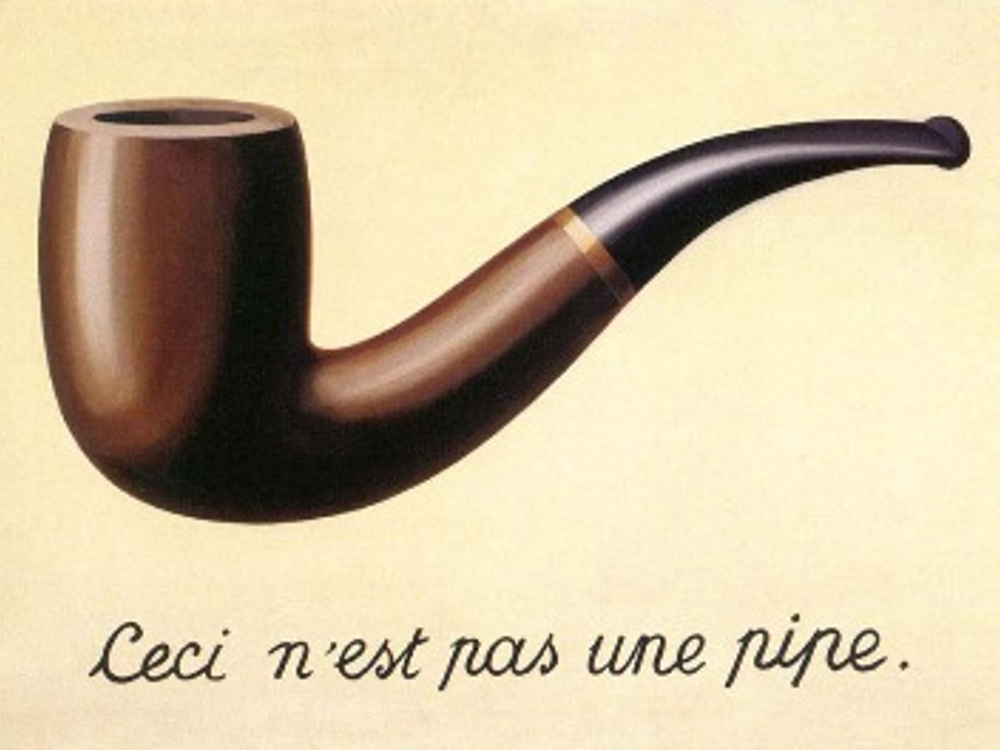
\includegraphics{streamlining-with-magrittr.jpg}

\end{frame}

\begin{frame}[fragile]{magrittr}
\protect\hypertarget{magrittr-1}{}

\begin{tikzpicture}[remember picture,overlay]
  \node[anchor=south west,inner sep=0pt] at ($(current page.south west)+(0cm,7.8cm)$) {
     
\includegraphics[width=1.5cm]{magrittr_log.jpg}
  };
\end{tikzpicture}

\begin{itemize}
\tightlist
\item
  Es el \emph{pipe} de R.
\item
  El uso es exactamente igual al `\textbar{}' de Bash.
\item
  Un único detalle: se utiliza \textbf{.} para hacer referencia a
  resultados intermedios en un pipe.
\end{itemize}

\begin{Shaded}
\begin{Highlighting}[]
\CommentTok{# hacer operaciones con una columna sin magrittr.}

\CommentTok{# Forma 1}
\NormalTok{Sepal.Width =}\StringTok{ }\NormalTok{iris}\OperatorTok{$}\NormalTok{Sepal.Width}
\NormalTok{Sepal.Width.Median =}\StringTok{ }\KeywordTok{median}\NormalTok{(Sepal.Width)}

\CommentTok{# Forma 2}
\NormalTok{Sepal.Width.Median =}\StringTok{  }\KeywordTok{median}\NormalTok{(iris}\OperatorTok{$}\NormalTok{Sepal.Width)}
\end{Highlighting}
\end{Shaded}

\begin{Shaded}
\begin{Highlighting}[]
\CommentTok{# con magrittr}
\KeywordTok{library}\NormalTok{(magrittr)}

\NormalTok{Sepal.Width.Median =}\StringTok{ }\NormalTok{iris }\OperatorTok\StringTok{ }\NormalTok{.}\OperatorTok{$}\NormalTok{Sepal.Width }\OperatorTok\StringTok{ }\KeywordTok{median}\NormalTok{(.) }
\end{Highlighting}
\end{Shaded}

\end{frame}

\begin{frame}{dpl}
\protect\hypertarget{dpl}{}

\begin{tikzpicture}[remember picture,overlay]
  \node[anchor=south west,inner sep=0pt] at ($(current page.south west)+(0cm,7.8cm)$) {
     
\includegraphics[width=1.5cm]{dplyr.png}
  };
\end{tikzpicture}


\includegraphics{filtro_filas.png}


\includegraphics{filtro_columna.png}

\end{frame}

\begin{frame}{}
\protect\hypertarget{section}{}

\begin{tikzpicture}[remember picture,overlay]
  \node[anchor=south west,inner sep=0pt] at ($(current page.south west)+(0cm,7.8cm)$) {
     
\includegraphics[width=1.5cm]{dplyr.png}
  };
\end{tikzpicture}

\begin{center}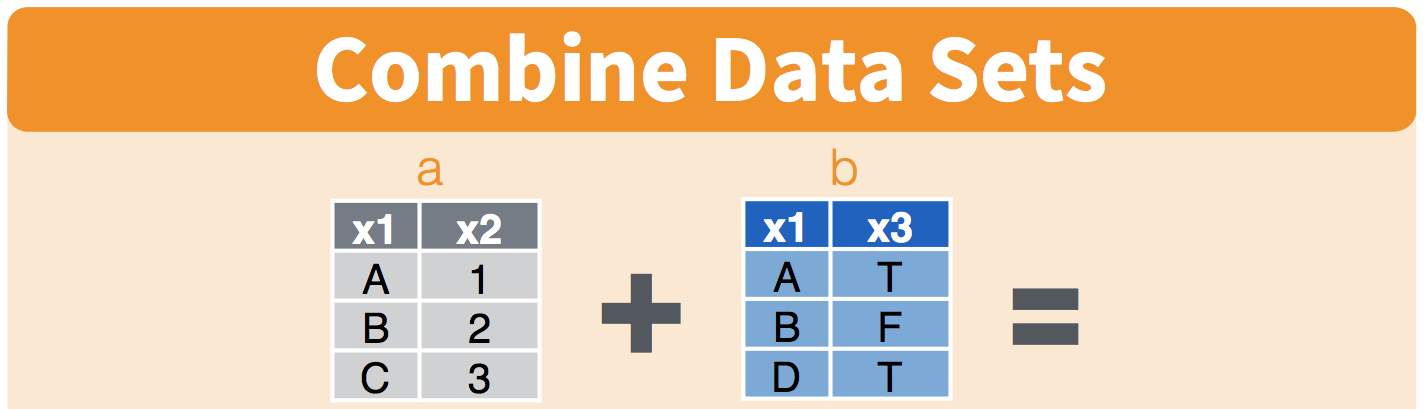
\includegraphics[width=0.5\linewidth]{combinando_dplyr} \end{center}

\begin{flushleft}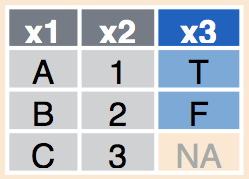
\includegraphics[width=0.2\linewidth]{comb_dplyr1} \end{flushleft}

\begin{flushleft}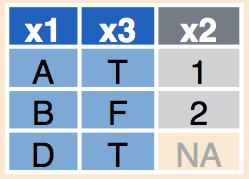
\includegraphics[width=0.2\linewidth]{comb_dplyr2} \end{flushleft}

\begin{flushright}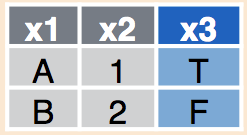
\includegraphics[width=0.2\linewidth]{comb_dplyr3} \end{flushright}

\begin{flushright}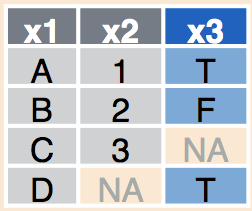
\includegraphics[width=0.2\linewidth]{comb_dplyr4} \end{flushright}

\end{frame}

\begin{frame}{tidyr}
\protect\hypertarget{tidyr}{}

\begin{tikzpicture}[remember picture,overlay]
  \node[anchor=south west,inner sep=0pt] at ($(current page.south west)+(0cm,7.8cm)$) {
     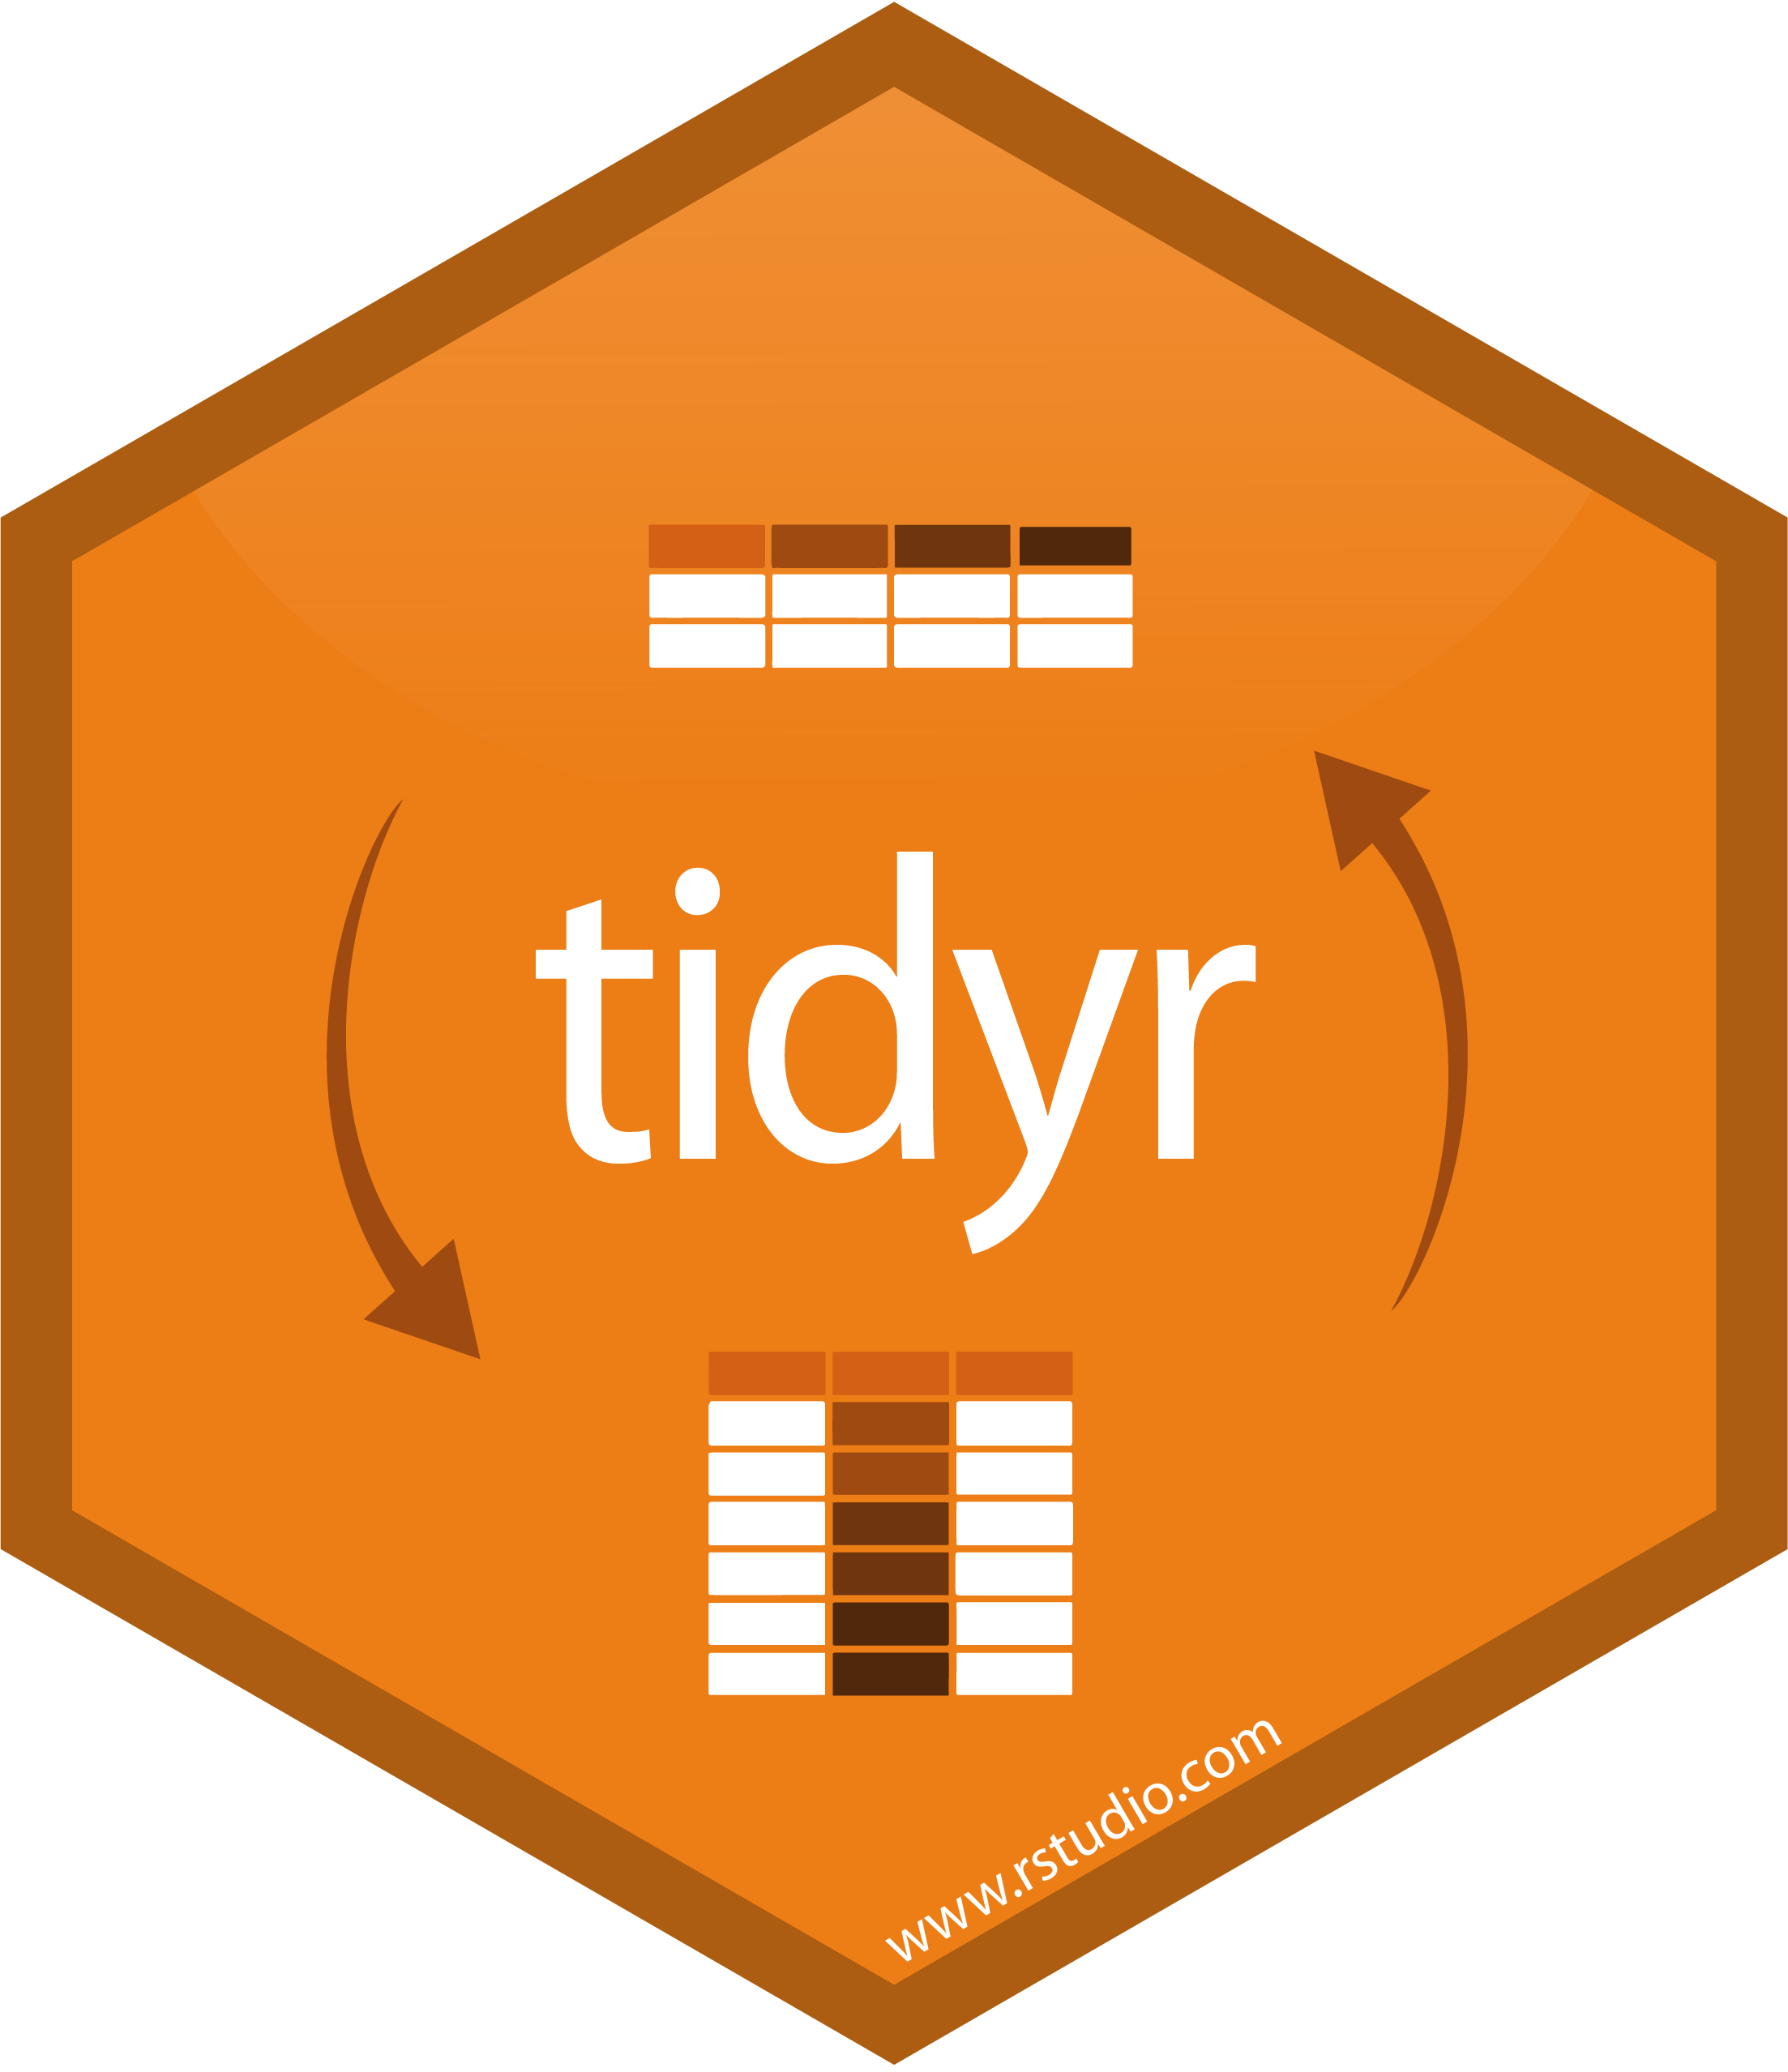
\includegraphics[width=1.5cm]{tidyr.png}
  };
\end{tikzpicture}

\begin{flushright}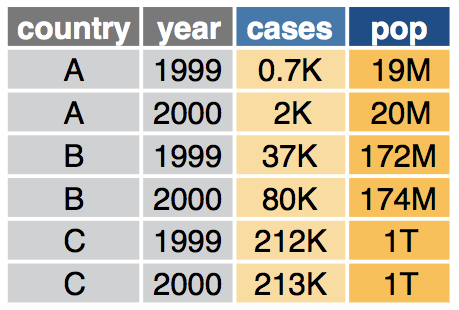
\includegraphics{data_wide} \end{flushright}

\begin{flushright}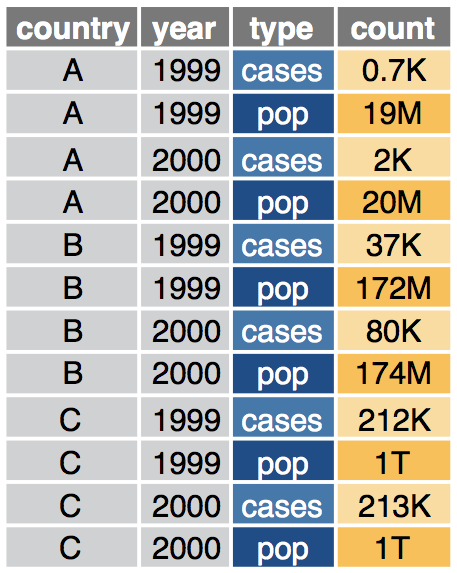
\includegraphics{data_long} \end{flushright}

\end{frame}

\begin{frame}{}
\protect\hypertarget{section-1}{}

\begin{flushright}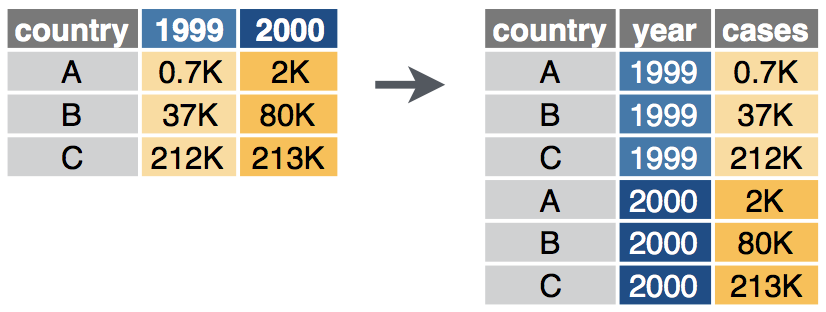
\includegraphics{pivot_longer_detailed} \end{flushright}

\begin{flushright}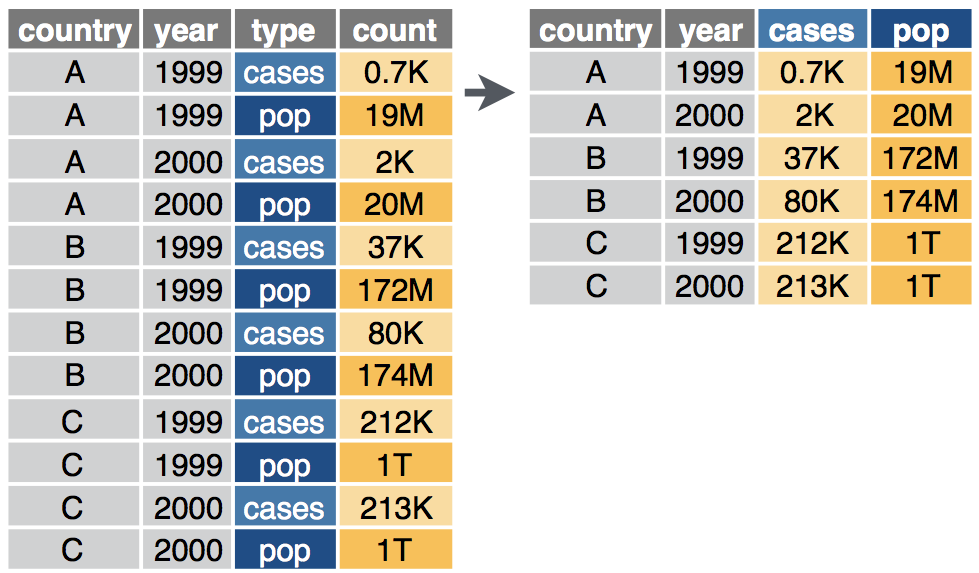
\includegraphics{pivot_wider_detailed} \end{flushright}

\end{frame}

\begin{frame}[fragile]{tidyr}
\protect\hypertarget{tidyr-1}{}

\begin{itemize}
\tightlist
\item
  You can represent the same underlying data in multiple ways. → ta
  bueno para mostrar diferentes tipos de datos \textbf{y decir por que
  esto es importante}.
\end{itemize}

\begin{verbatim}
## # A tibble: 150 x 5
##    Sepal.Length Sepal.Width Petal.Length Petal.Width Species
##           <dbl>       <dbl>        <dbl>       <dbl> <fct>  
##  1          5.1         3.5          1.4         0.2 setosa 
##  2          4.9         3            1.4         0.2 setosa 
##  3          4.7         3.2          1.3         0.2 setosa 
##  4          4.6         3.1          1.5         0.2 setosa 
##  5          5           3.6          1.4         0.2 setosa 
##  6          5.4         3.9          1.7         0.4 setosa 
##  7          4.6         3.4          1.4         0.3 setosa 
##  8          5           3.4          1.5         0.2 setosa 
##  9          4.4         2.9          1.4         0.2 setosa 
## 10          4.9         3.1          1.5         0.1 setosa 
## # ... with 140 more rows
\end{verbatim}

\end{frame}

\begin{frame}[fragile]{tidyr}
\protect\hypertarget{tidyr-2}{}

\begin{verbatim}
## # A tibble: 600 x 3
##    Species Variable     value
##    <fct>   <chr>        <dbl>
##  1 setosa  Sepal.Length   5.1
##  2 setosa  Sepal.Width    3.5
##  3 setosa  Petal.Length   1.4
##  4 setosa  Petal.Width    0.2
##  5 setosa  Sepal.Length   4.9
##  6 setosa  Sepal.Width    3  
##  7 setosa  Petal.Length   1.4
##  8 setosa  Petal.Width    0.2
##  9 setosa  Sepal.Length   4.7
## 10 setosa  Sepal.Width    3.2
## # ... with 590 more rows
\end{verbatim}

\end{frame}

\begin{frame}[fragile]{tidyr}
\protect\hypertarget{tidyr-3}{}

\begin{itemize}
\tightlist
\item
  There are three interrelated rules which make a dataset tidy:
\end{itemize}

\begin{enumerate}
\tightlist
\item
  Each variable must have its own column.
\item
  Each observation must have its own row.
\item
  Each value must have its own cell.
\end{enumerate}

\begin{itemize}
\item
  {[}\textbf{most real world data is untidy}{]} This means for most real
  analyses, you'll need to do some tidying. The first step is always to
  figure out what the variables and observations are.
\item
  The second step is to resolve one of two common problems:

  \begin{enumerate}
  \tightlist
  \item
    One variable might be spread across multiple columns.
  \item
    One observation might be scattered across multiple rows.
  \end{enumerate}
\item
  Typically a dataset will only suffer from one of these problems; it'll
  only suffer from both if you're really unlucky! To fix these problems,
  \textbf{you'll need the two most important functions in tidyr}:
  \texttt{pivot\_longer()} and \texttt{pivot\_wider()}.
\item
  A common problem is a dataset where some of the column names are not
  names of variables, but values of a variable. Take table4a: the column
  names 1999 and 2000 represent values of the year variable, the values
  in the 1999 and 2000 columns represent values of the cases variable,
  and each row represents two observations, not one.
\item
  To tidy a dataset like this, we need to pivot the offending columns
  into a new pair of variables. To describe that operation we need three
  parameters:

\begin{verbatim}
  table4a %>%
      pivot_longer(c(`1999`, `2000`), names_to = "year", values_to = "cases")
\end{verbatim}
\end{itemize}

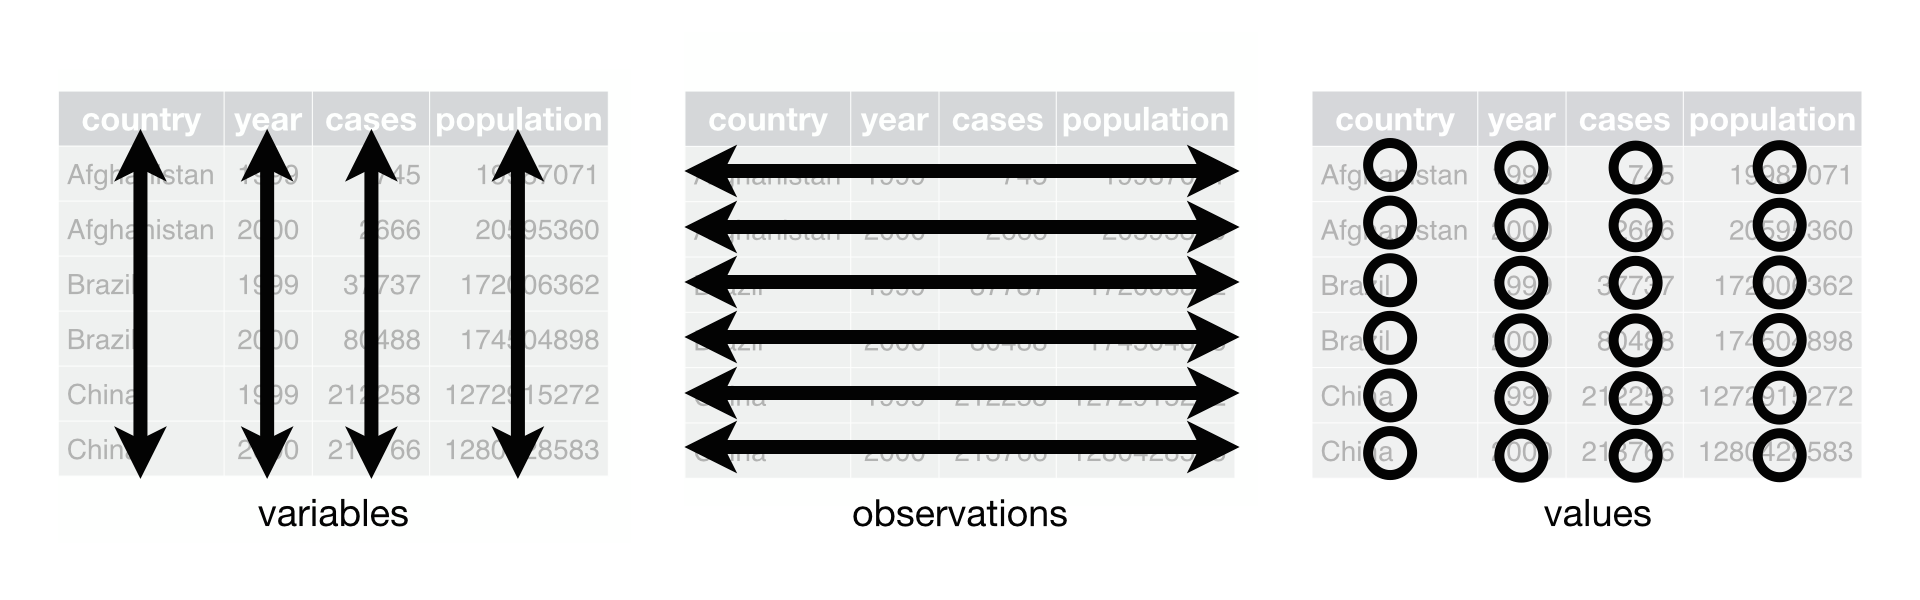
\includegraphics{tidy-1.png}

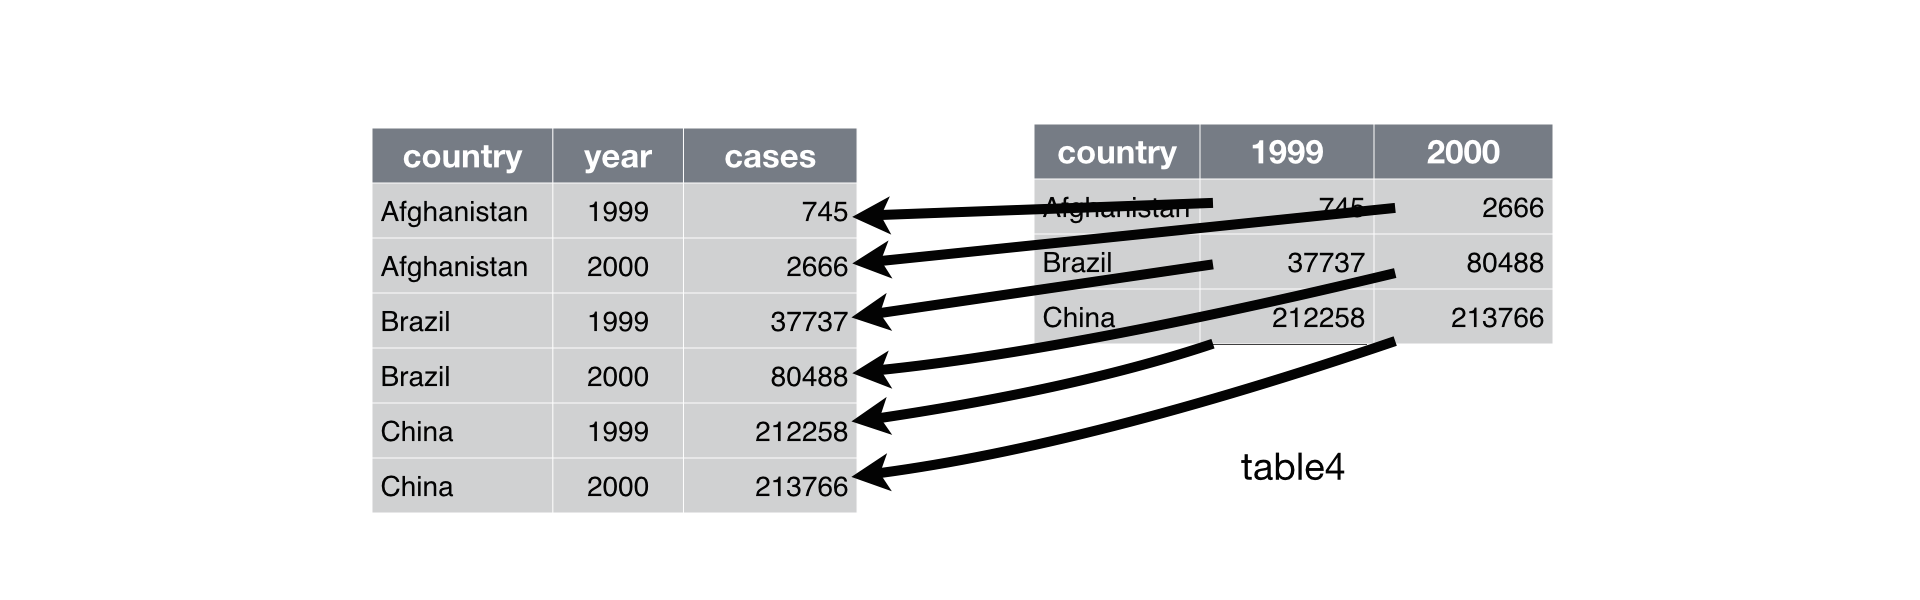
\includegraphics{tidy-9.png}

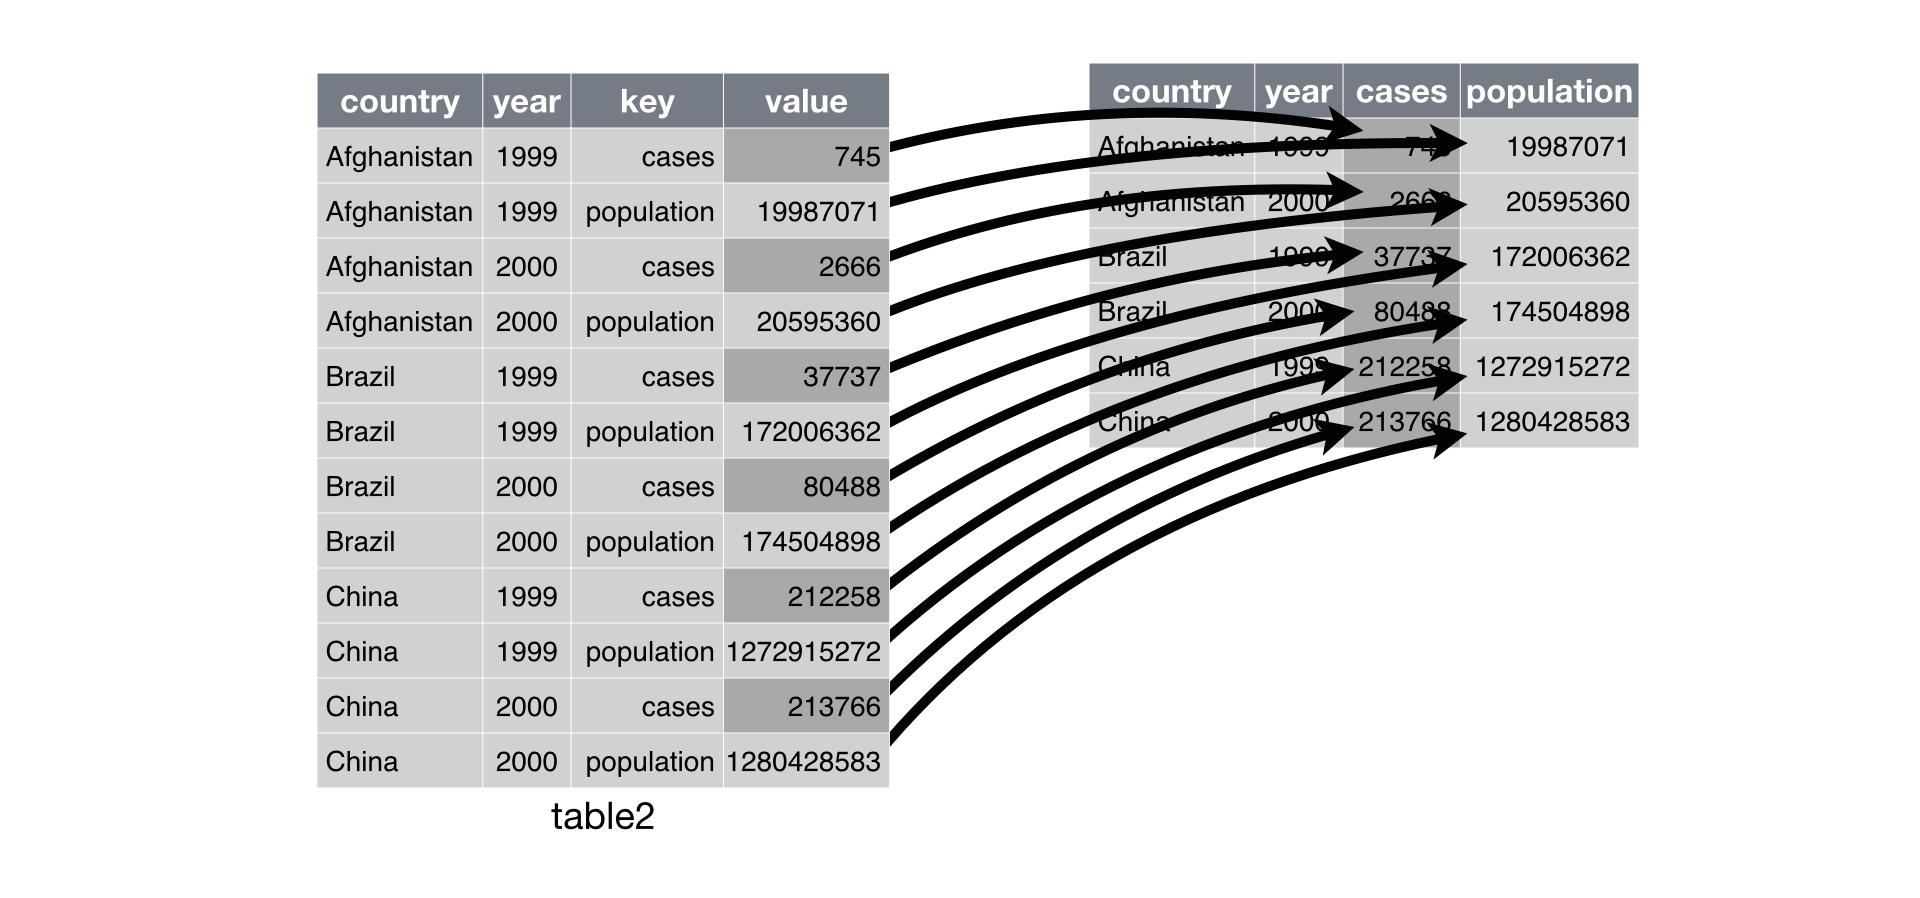
\includegraphics{tidy-8.png}

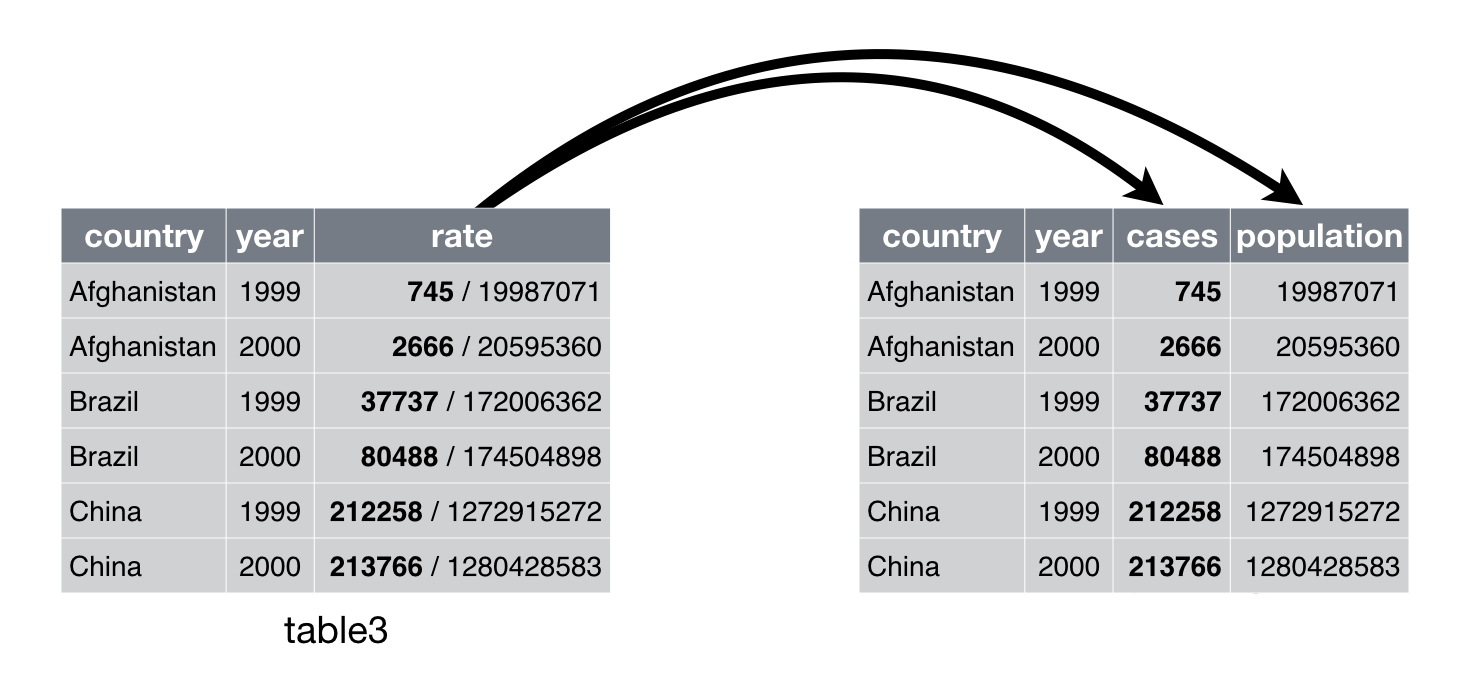
\includegraphics{tidy-17.png}

\end{frame}

\begin{frame}{gg}
\protect\hypertarget{gg}{}

\begin{tikzpicture}[remember picture,overlay]
  \node[anchor=south west,inner sep=0pt] at ($(current page.south west)+(0cm,7.8cm)$) {
     
\includegraphics[width=1.5cm]{ggplot2_logo.png}
  };
\end{tikzpicture}

\begin{itemize}
\tightlist
\item
  Es importante aca explicar cosas como lo de \textbf{aes()} y cosas del
  estilo. Para eso hay que leer bien un articulo sobre ggplot2!
\end{itemize}

\end{frame}

\begin{frame}{}
\protect\hypertarget{section-2}{}

\begin{tikzpicture}[remember picture,overlay]
  \node[anchor=south west,inner sep=0pt] at ($(current page.south west)+(0cm,7.8cm)$) {
     
\includegraphics[width=1.5cm]{ggplot2_logo.png}
  };
\end{tikzpicture}

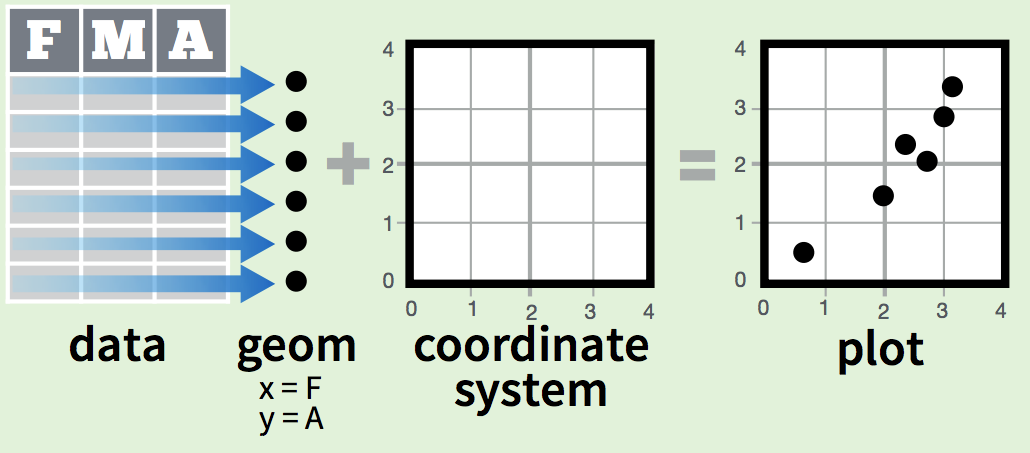
\includegraphics{ggplot_basico_1.png}

\end{frame}

\begin{frame}{}
\protect\hypertarget{section-3}{}

\begin{tikzpicture}[remember picture,overlay]
  \node[anchor=south west,inner sep=0pt] at ($(current page.south west)+(0cm,7.8cm)$) {
     
\includegraphics[width=1.5cm]{ggplot2_logo.png}
  };
\end{tikzpicture}

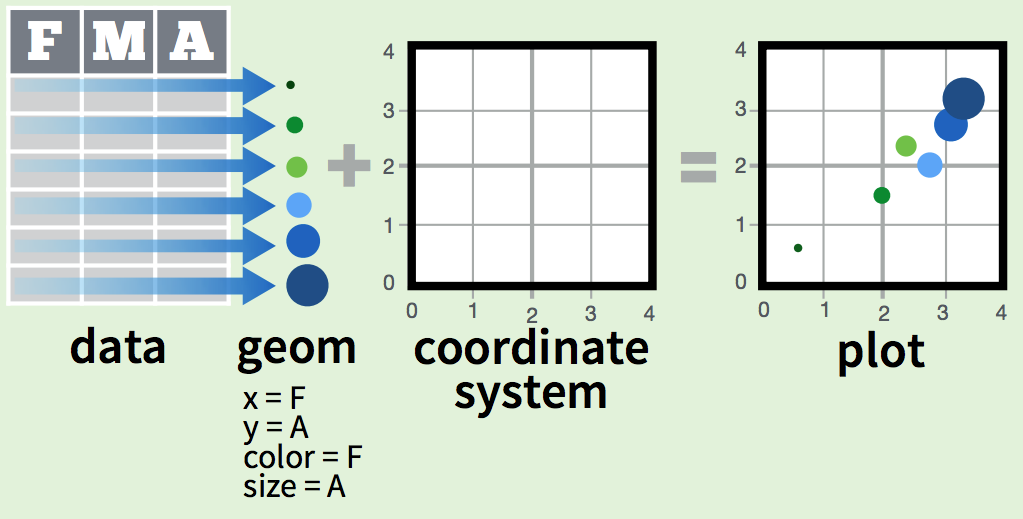
\includegraphics{ggplot_basico_2.png}

\end{frame}

\begin{frame}{}
\protect\hypertarget{section-4}{}

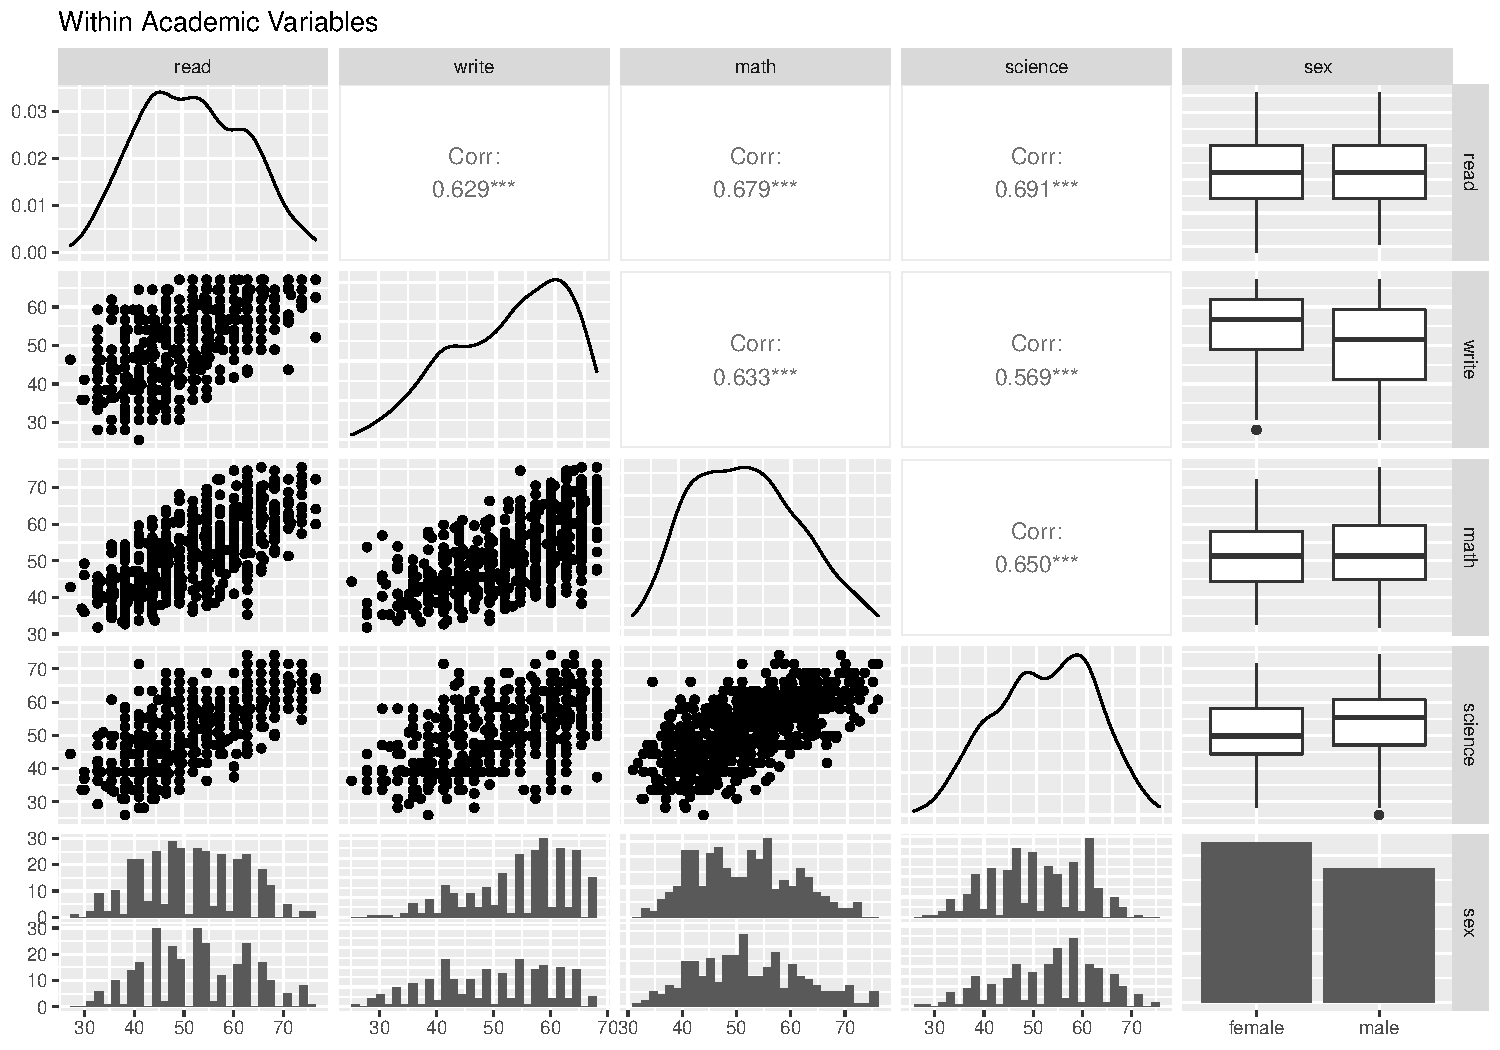
\includegraphics{claseIntro_practico12_files/figure-beamer/unnamed-chunk-31-1.pdf}

\end{frame}

\begin{frame}[fragile]{Una ventaja: reproduclbilidad}
\protect\hypertarget{una-ventaja-reproduclbilidad}{}

\begin{Shaded}
\begin{Highlighting}[]
\KeywordTok{library}\NormalTok{(tidyverse)}

\CommentTok{# se utiliza el set de datos iris}
\NormalTok{iris }\OperatorTok
\StringTok{  }\CommentTok{# se grafica Sepal.Length vs Sepal.Width,}
\StringTok{  }\CommentTok{# coloreando segun Species}
\StringTok{  }\KeywordTok{ggplot}\NormalTok{(}\DataTypeTok{data =}\NormalTok{ .,}
          \KeywordTok{aes}\NormalTok{(}\DataTypeTok{x =}\NormalTok{ Sepal.Length, }
              \DataTypeTok{y =}\NormalTok{ Sepal.Width, }
              \DataTypeTok{color =}\NormalTok{ Species, }
              \DataTypeTok{fill =}\NormalTok{ Species)) }\OperatorTok{+}
\StringTok{  }\CommentTok{# se grafica utilizando puntos}
\StringTok{  }\KeywordTok{geom_point}\NormalTok{() }\OperatorTok{+}\StringTok{ }
\StringTok{  }\CommentTok{# se separa el set de datos segun Species}
\StringTok{  }\KeywordTok{facet_wrap}\NormalTok{(}\OperatorTok{~}\NormalTok{Species)}
\end{Highlighting}
\end{Shaded}

\end{frame}

\begin{frame}[fragile]{Otra ventaja: fácil modificación}
\protect\hypertarget{otra-ventaja-fuxe1cil-modificaciuxf3n}{}

\begin{Shaded}
\begin{Highlighting}[]
\KeywordTok{library}\NormalTok{(tidyverse)}

\CommentTok{# se utiliza el set de datos iris}
\NormalTok{iris }\OperatorTok
\StringTok{  }\CommentTok{# se grafica Sepal.Length vs Sepal.Width,}
\StringTok{  }\CommentTok{# coloreando segun Species}
\StringTok{  }\KeywordTok{ggplot}\NormalTok{(}\DataTypeTok{data =}\NormalTok{ .,}
          \KeywordTok{aes}\NormalTok{(}\DataTypeTok{x =}\NormalTok{ Sepal.Length, }
              \DataTypeTok{y =}\NormalTok{ Sepal.Width, }
              \DataTypeTok{color =}\NormalTok{ Species, }
              \DataTypeTok{fill =}\NormalTok{ Species)) }\OperatorTok{+}
\StringTok{  }\CommentTok{# se grafica utilizando puntos}
\StringTok{  }\KeywordTok{geom_point}\NormalTok{() }\OperatorTok{+}\StringTok{ }
\CommentTok{#  # se separa el set de datos segun Species}
\CommentTok{#  facet_wrap(~Species)}
\end{Highlighting}
\end{Shaded}

\end{frame}

\begin{frame}{Otra ventaja: fácil modificación}
\protect\hypertarget{otra-ventaja-fuxe1cil-modificaciuxf3n-1}{}

\includegraphics{claseIntro_practico12_files/figure-beamer/unnamed-chunk-34-1.pdf}

\end{frame}

\begin{frame}{¿Donde encuentro info sobre estos paquetes?}
\protect\hypertarget{donde-encuentro-info-sobre-estos-paquetes}{}

\begin{itemize}
\tightlist
\item
  Cheatsheets
\item
  Vignettes
\end{itemize}

\end{frame}

\begin{frame}{Otros ejemplos}
\protect\hypertarget{otros-ejemplos}{}

\end{frame}

\begin{frame}{Estadística: análisis multivariado}
\protect\hypertarget{estaduxedstica-anuxe1lisis-multivariado}{}

\end{frame}

\begin{frame}{Clustering: librería pheatmap}
\protect\hypertarget{clustering-libreruxeda-pheatmap}{}

\end{frame}

\begin{frame}{GGally}
\protect\hypertarget{ggally}{}

\end{frame}

\begin{frame}{Filogenética: librería ggtree}
\protect\hypertarget{filogenuxe9tica-libreruxeda-ggtree}{}

\includegraphics{claseIntro_practico12_files/figure-beamer/unnamed-chunk-35-1.pdf}

\end{frame}

\begin{frame}{Genómica: BioCircos/rcirclize y gggnomics, ggbio}
\protect\hypertarget{genuxf3mica-biocircosrcirclize-y-gggnomics-ggbio}{}

\end{frame}

\begin{frame}{Biología estructural:}
\protect\hypertarget{biologuxeda-estructural}{}

\end{frame}

\begin{frame}{Espectrometria de masas}
\protect\hypertarget{espectrometria-de-masas}{}

\end{frame}

\begin{frame}{Ecologia}
\protect\hypertarget{ecologia}{}

\end{frame}

\end{document}
